\chapter{Конструкторская часть}

В данном разделе представлены этапы проектирования выделенных в предыдущем разделе баз данных, нужных для решения задачи.

\section{Проектирование отношений сущностей}

На рисунке \ref{img:arch} представлена схема сущностей, необходимых для реализации приложения.

\begin{figure}[h!]
	\begin{center}
		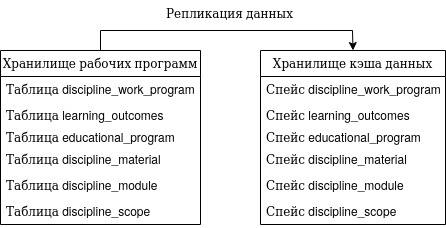
\includegraphics[scale=0.5]{img/arch.jpg}
	\end{center}
	\captionsetup{justification=centering}
	\caption{Схема сущностей приложения}
	\label{img:arch}
\end{figure}

\section{Проектирование базы данных рабочих программ дисциплин}

База данных рабочих программ дисциплин будет реализована с использованием СУБД PostgreSQL. В базе данных будет существовать 6 сущностей и 7 таблиц, одна из которых является развязочной. ER-диаграма сущностей этой базы данных представлена на рисунке \ref{img:er-storage}.\\

\begin{figure}[h!]
	\begin{center}
		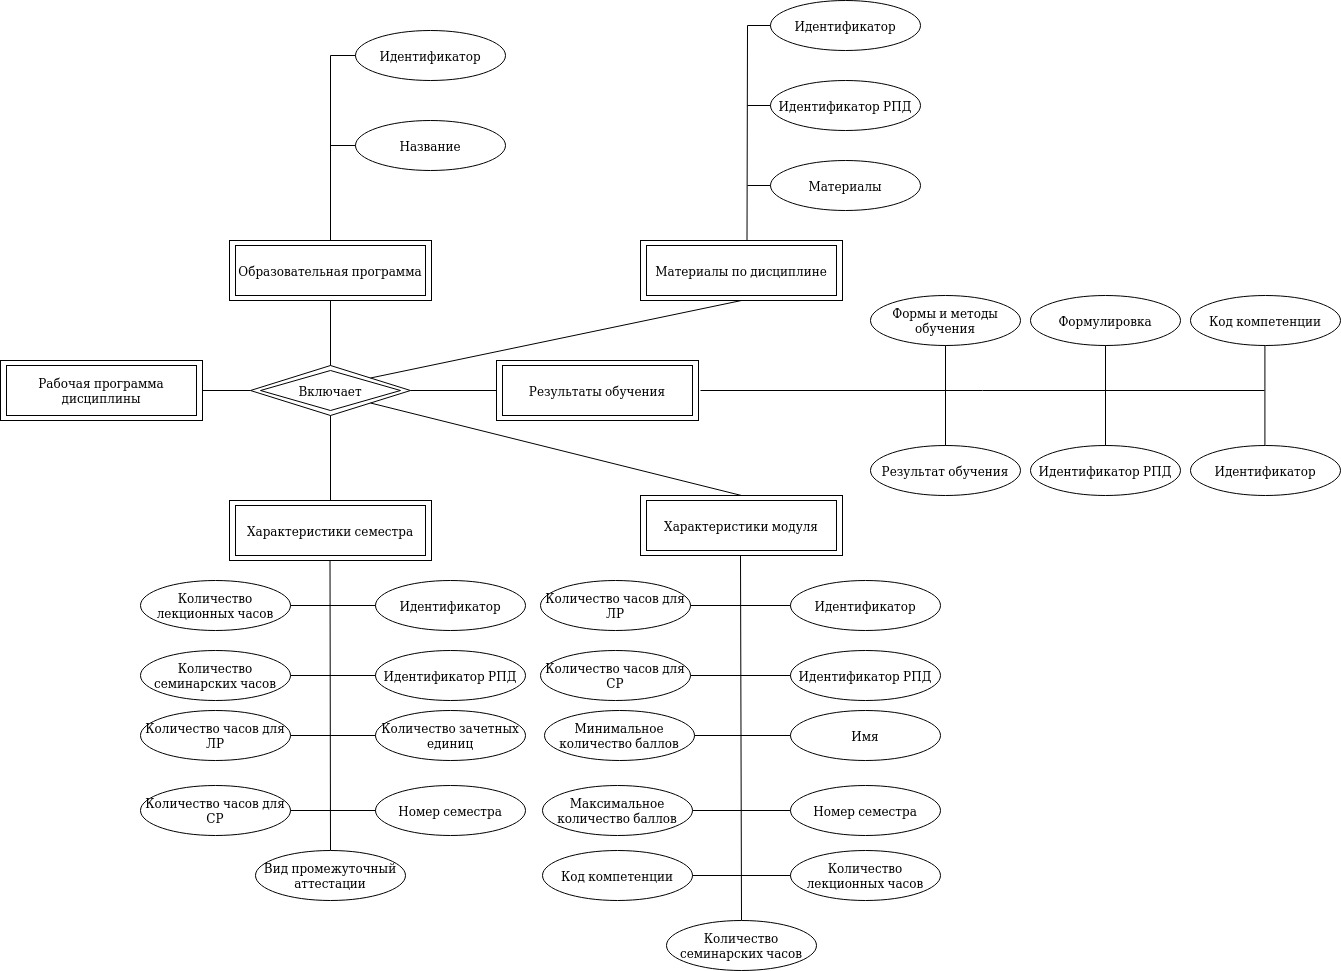
\includegraphics[scale=0.35]{img/er-chen.jpg}
	\end{center}
	\captionsetup{justification=centering}
	\caption{ER-диаграмма сущностей базы данных рабочих программ дисциплин в нотации Чена}
	\label{img:er-storage}
\end{figure}

Поля таблицы \texttt{discipline\_work\_program} означают:

\begin{itemize}
	\item \texttt{id} -- уникальный идентификатор рабочей программы дисциплин; будет использоваться чтобы однозначно идентифицировать рабочую программу в системе;
	\item \texttt{name} -- название дисциплины;
	\item \texttt{author} -- ФИО автора рабочей программы дисциплины; 
	\item \texttt{competency} -- компетенция рабочей программы.
\end{itemize}

Данная таблица является ключевой и имеет связи с другими таблицами с отношением один-ко-многим и многие-ко-многим. Такая схема хранения хранить получить всю информацию о дисциплине, зная лишь ее уникальный идентификатор. При этом, такая схема хранения является достаточно гибкой.\\

Таблица \texttt{educational\_program} хранит информацию о образовательной программе:

\begin{itemize}
	\item \texttt{id} -- уникальный идентификатор образовательной программы;
	\item \texttt{name} -- имя образовательной программы.
\end{itemize}
 
Данная таблица и таблица \texttt{discipline\_work\_program} имеет отношение многие-ко-многим. Например, дисциплина <<Объектно ориентированное программирование>> преподается на образовательной программе <<Программная инженерия>> и <<Информационная аналитика и политические технологии>>.\\

Таблица \texttt{learning\_outcomes} содержит информацию о результатах обучения по данной дисциплине:

\begin{itemize}
	\item \texttt{id} -- уникальный идентификатор таблицы;
	\item \texttt{discipline\_id} -- внешний ключ для таблицы \texttt{discipline\_work\_program};
	\item \texttt{competency\_code} -- код компетенции;
	\item \texttt{formulation} -- формулировка компетенции;
	\item \texttt{results} -- результаты обучения;
	\item \texttt{forms\_and\_methods} -- формы и методы обучения.
\end{itemize}

Эта таблица имеет связь с таблицей \texttt{discipline\_work\_program} c отношением один-ко-многим. У дисциплины для каждого направления подготовки должны быть различные результаты обучения.\\

Таблица \texttt{discipline\_scope} содержит информацию о объеме дисциплины для каждого семестра:

\begin{itemize}
	\item \texttt{id} -- уникальный идентификатор таблицы;
	\item \texttt{discipline\_id} -- внешний ключ для таблицы \texttt{discipline\_work\_program};
	\item \texttt{semester\_number} -- номер семестра;
	\item \texttt{credit\_units} -- количество зачетных единиц;
	\item \texttt{total\_hours} -- общее количество часов;
	\item \texttt{lectures\_hours} -- количество часов, выделенных для проведения лекций;
	\item \texttt{seminars\_hours} -- количество часов, выделенных на семинарские занятия;
	\item \texttt{laboratory\_work\_hours} -- количество часов, выделенное на лабораторные работы;
	\item \texttt{independent\_work\_hours} -- количество часов, выделенное на самостоятельную работу студентом;
	\item \texttt{certification\_type} -- вид промежуточный аттестации -- экзамен или зачет.
\end{itemize}

Эта таблица имеет связь с таблицей \texttt{discipline\_work\_program} c отношением один-ко-многим. Дисциплина может преподаваться несколько семестров.\\

Таблица \texttt{discipline\_module} содержит информацию о содержании дисциплины для каждого модуля учебной дисциплины:

\begin{itemize}
	\item \texttt{id} -- уникальный идентификатор таблицы;
	\item \texttt{discipline\_id} -- внешний ключ для таблицы \texttt{discipline\_work\_program};
	\item \texttt{semester\_number} -- номер семестра;
	\item \texttt{name} -- название модуля;
	\item \texttt{credit\_units} -- количество зачетных единиц;
	\item \texttt{total\_hours} -- общее количество часов;
	\item \texttt{lectures\_hours} -- количество часов, выделенных для проведения лекций;
	\item \texttt{seminars\_hours} -- количество часов, выделенных на семинарские занятия;
	\item \texttt{laboratory\_work\_hours} -- количество часов, выделенное на лабораторные работы;
	\item \texttt{independent\_work\_hours} -- количество часов, выделенное на самостоятельную работу студентом;
	\item \texttt{min\_scores} -- минимальное количество баллов, которое нужно набрать обучающемуся для закрытия этого модуля;
	\item \texttt{max\_scores} -- максимальное количество баллов, которое можно набрать в течении этого модуля;
	\item \texttt{competency\_codes} -- компетенции, закрепленные за темой.
\end{itemize}

Эта таблица имеет связь с таблицей \texttt{discipline\_work\_program} c отношением один-ко-многим. Дисциплина чаще всего имеет несколько модулей.\\

Таблица \texttt{discpline\_material} содержит сведение о материалах, необходимых для освоения дисциплины:

\begin{itemize}
	\item \texttt{id} -- уникальный идентификатор таблицы;
	\item \texttt{discipline\_id} -- внешний ключ для таблицы \texttt{discipline\_work\_program};
	\item \texttt{material\_id} -- литература, необходимая для освоения дисциплины;
\end{itemize}

Эта таблица имеет связь с таблицей \texttt{discipline\_work\_program} c отношением один-ко-многим. Для освоения дисциплины, обычно, необходимо более чем один источник информации.\\

Кроме того, для каждой таблицы будет реализован триггер, срабатывающий после обновления или удаления данных из таблиц. Этот триггер будет посылать сигнал базе данных кэширования, с помощью языка plpython3u, о необходимости обновить или удалить информацию из кэша. С помощью таких триггеров можно решить проблему синхронизации данных в хранилище и кэше.

\section{Проектирование базы данных кэширования}

База данных кэширования будет реализована с помощью использования СУБД Tarantool. В базе данных будут полностью продублированны таблицы (в виде спейсов) из хранилища рабочих программ дисциплин. Первичным ключом будет являться поле с уникальным идентификатором этих таблиц (\texttt{id}). Кроме того, для спейсов хранящих поле \texttt{discipline\_id} будет добавлен вторичный ключ по этому полю, для удобного и быстрого сбора нужных данных по заданной дисциплине.

При запросе данных у приложения, будет проводиться проверка, присутствует ли запись в кэше. Если запись присутствует, запрос к базе данных рабочих программ дисциплин производиться не будет и будут возвращены данные из кэша. В противном случае, будет произведен запрос к базе данных хранящую информацию о дисциплинах.

Все спейсы будут созданы на основе движка \texttt{memtx}, хранящего все данные в оперативной памяти. Персистентность данных будет обеспечивается при помощи ведения журнала транзакция и системы <<снимков>> текущего состояния кэша. Эти технологии помогут решить проблему <<холодного>> старта базы данных кэширования.

\section*{Вывод}

В данном разделе были представлены этапы проектирования баз данных и рассмотрены особенности используемых СУБД на архитектурном уровне.
